In this section we define the attacker model and show the security guarantees given by \lang. Specifically, we show that \lang{} executions satisfy termination-insensitive noninterference \cite{4223226}. Formally, an attacker is some principal $\Attacker$. Note that this principal might be a conjunction of named principals $n_1 \wedge \dots \wedge n_k$ representing a set of $k$ colluding principals. In the sections that follow we denote a $\Nameset$-indexed set of memories as a function $\globalstore: \Nameset \to (\Addr \partialto \val)$.

\subsection{Trace semantics}
We express the attacker model in terms of a trace semantics, in which certain operations in the language emit \emph{events} which may or may not be observable by $\Attacker$. The grammar for events is given in Figure~\ref{fig:event-syntax}. These event should be self-explanatory, with the exception of $\mathsf{release}$ events, which we explain later in this section. An non-empty event $\event$ contains the type of the event, the current environment when the event was emitted, and the node that emitted the event. An attacker observes modifications to memory (ie., writes or allocations) locally on a machine and remote procedure calls and returns across machines. This choice correspond to a typical Dolev-Yao attacker model \cite{Dolev:1981:SPK:1382435.1382728}.

\begin{figure}
\centering
\begin{align*}
\event &::= (\alpha, \env, n) \mid \varepsilon\\
\alpha &::= \mathsf{write}(\addr, \expr) \mid \mathsf{new}(\addr, \expr) \mid \mathsf{call}(\expr, n) \\ &\quad \mid \mathsf{ret}(\val, n) \mid \mathsf{stop}(\val, n) \mid \mathsf{release}(p, q, r)
\end{align*}
\caption{The syntax of events.}
\label{fig:event-syntax}
\end{figure}

We call a sequence of events a trace. We write the concatenation of traces as $t_1 \cdot t_2$ and we write the empty trace as $\varepsilon$. Given a trace $t$ the observable trace of $t$ is the trace $t \upharpoonright \Attacker$, defined as
\begin{align*}
\varepsilon \upharpoonright \Attacker &= \varepsilon\\
((\alpha, \env, n) \cdot t) \upharpoonright \Attacker &=
\begin{cases}
(\alpha, \env, n) \cdot (t \upharpoonright \Attacker) & \nopostflowstoquery{n; \env}{\env_n.\lblkw}{\Attacker} \\
t \upharpoonright \Attacker & \text{otherwise}
\end{cases}
\end{align*}
We augment the semantics from Section~\ref{sec:calculus} with events. Figure~\ref{fig:event-semantics} shows an excerpt of the augmented semantics. Except for the emitted event these rules correspond exactly to the rules in Figure~\ref{fig:monadic-reductions} and Figure~\ref{fig:global-steps}. It will be convenient to write $\gconfig{n}{\env}{S} \gstepstos[][t]$ when there exists a configuration $\gconfig{n'}{\env'}{S'}$ such that $\gconfig{n}{\env}{S} \gstepstos[][t] \gconfig{n'}{\env'}{S'}$. We also write $\gconfig{n}{\env}{S} \gstepstos[][\Attacker \filtertrace t']$ when $\gconfig{n}{\env}{S} \gstepstos[][t]$ and $t' = \Attacker \upharpoonright t$.

\begin{figure}
\centering
\begin{mathpar}
\inferrule[E-Write-Ev]{\store(\addr) = \lb{p}{\expr} \and \flowstoquery{n; \env}{\env_n.\lblkw}{p \flowsto n}{\level} \\\\ \nopostflowstoquery{n; \env}{\env_n.\lblkw \join \level}{n} \and \store' = \extend{\store}{\addr}{\lb{p}{\expr'}} \\\\ \sigma = \extend{\env_n}{\lblkw}{\env_n.\lblkw \join \level} \\\\ \event = (\mathsf{write}(\addr, \expr'), \env, n)}{\step{n; \env}[][\event]{\config{\store}{\efill{\writeref{\addr}{\expr'}}}}{ \config{\store'}{\efill{\return{()}}}}{\sigma}}
\and
\inferrule[G-Step-Ret-Ev]{S_n = \config{\store_n}{\efill{\wait{m}[\type]}} \and S_m = \config{\store_m}{\val ; \overline{\expr_m}} \\\\ \event = (\mathsf{ret}(\val, n), \env, m)}{\gconfig{m}{\env}{S} \gstepsto[][\event] \gconfig{n}{\env}{\extends{S}{n \mapsto \config{\store_n}{\efill{\val}}, m \mapsto \config{\store_m}{\overline{\expr_m}}}}}
\and
\inferrule[G-Step-Local-Ev]{\step{n; \env}[][\event]{S_n}{S'}{\sigma}}{\gconfig{n}{\env}{S} \gstepsto[][\event] \gconfig{n}{\extend{\env}{n}{\sigma}}{\extend{S}{n}{S'}}}
\and
\inferrule[E-Assume-Ev]{
\flowstoquery{n; \env}{\env_n.\lblkw}{r \flowsto n}{\level_1} \\\\ \actsforquery{n; \env}{\env_n.\lblkw}{\voice{q}}{\level_2} \\\\ \nopostflowstoquery{n; \env}{\env_n.\lblkw \join \level_1 \join \level_2}{n} \\\\ \sigma = \extends{\env_n}{\scope \mapsto \cons{\lb{r}{(p, q)}}{\env . \scope}), \lblkw \mapsto \env_n.\lblkw \join \level_1 \join \level_2} \\\\ \event = (\mathsf{release}(p, q, r), \env, n)}{\step{n; \env}[][\event]{\config{\store}{\efill{\adddelegate{p}{q}{r}}}}{ \config{\store}{\efill{\return{()}}}}{\sigma}}
\end{mathpar}
\caption{Augmented semantics emitting events.}
\label{fig:event-semantics}
\end{figure}

\paragraph{Release events}\label{sec:release-events}
In order to define noninterference we require that nodes agree on which principals flow to $\Attacker$. That is, it must not be the case that Alice considers data to not be observable by $\Attacker$, and then send it to Bob, who considers the same data to be observable by $\Attacker$. Relaxations of such limitations, like robust declassification \cite{Zdancewic:2001:RD:872752.873524, Myers:2004:ERD:1009380.1009673} and nonmalleable information-flow \cite{Cecchetti:2017:NIF:3133956.3134054}, is orthogonal to this work and we therefore consider only the case where nodes agree on which principals flow to $\Attacker$ in the information-flow lattice. To capture this intuition we introduce the notion of a ``good'' release event.

\paragraph{Good events}
We call a release event $\event = (\mathsf{release}(p, q, r), \env, n)$ good, written $\good{\Attacker}{\event}$, if $\nopostflowstoquery{n; \env}{r}{\Attacker}$ implies $\nopostflowstoquery{n; \env}{p}{\Attacker} \iff \nopostflowstoquery{n; \env}{q}{\Attacker}$. Intuitively, this means that any expression of the form $\adddelegate{p}{q}{r}$ such that $r$ flows to $\Attacker$ should not modify what the attacker can observe. An illustration capturing when a flow is not good is shown in Figure~\ref{fig:bad-release}. We extend the notion of good to traces and say a trace is good, written $\good{\Attacker}{t}$ if all release events in $t$ are good release events. Our noninterference result, presented at the end of this section, will quantify only over good traces, and we leave the problem of extending this result to more relaxed notions of noninterference as future work.

\begin{figure}
    \centering
    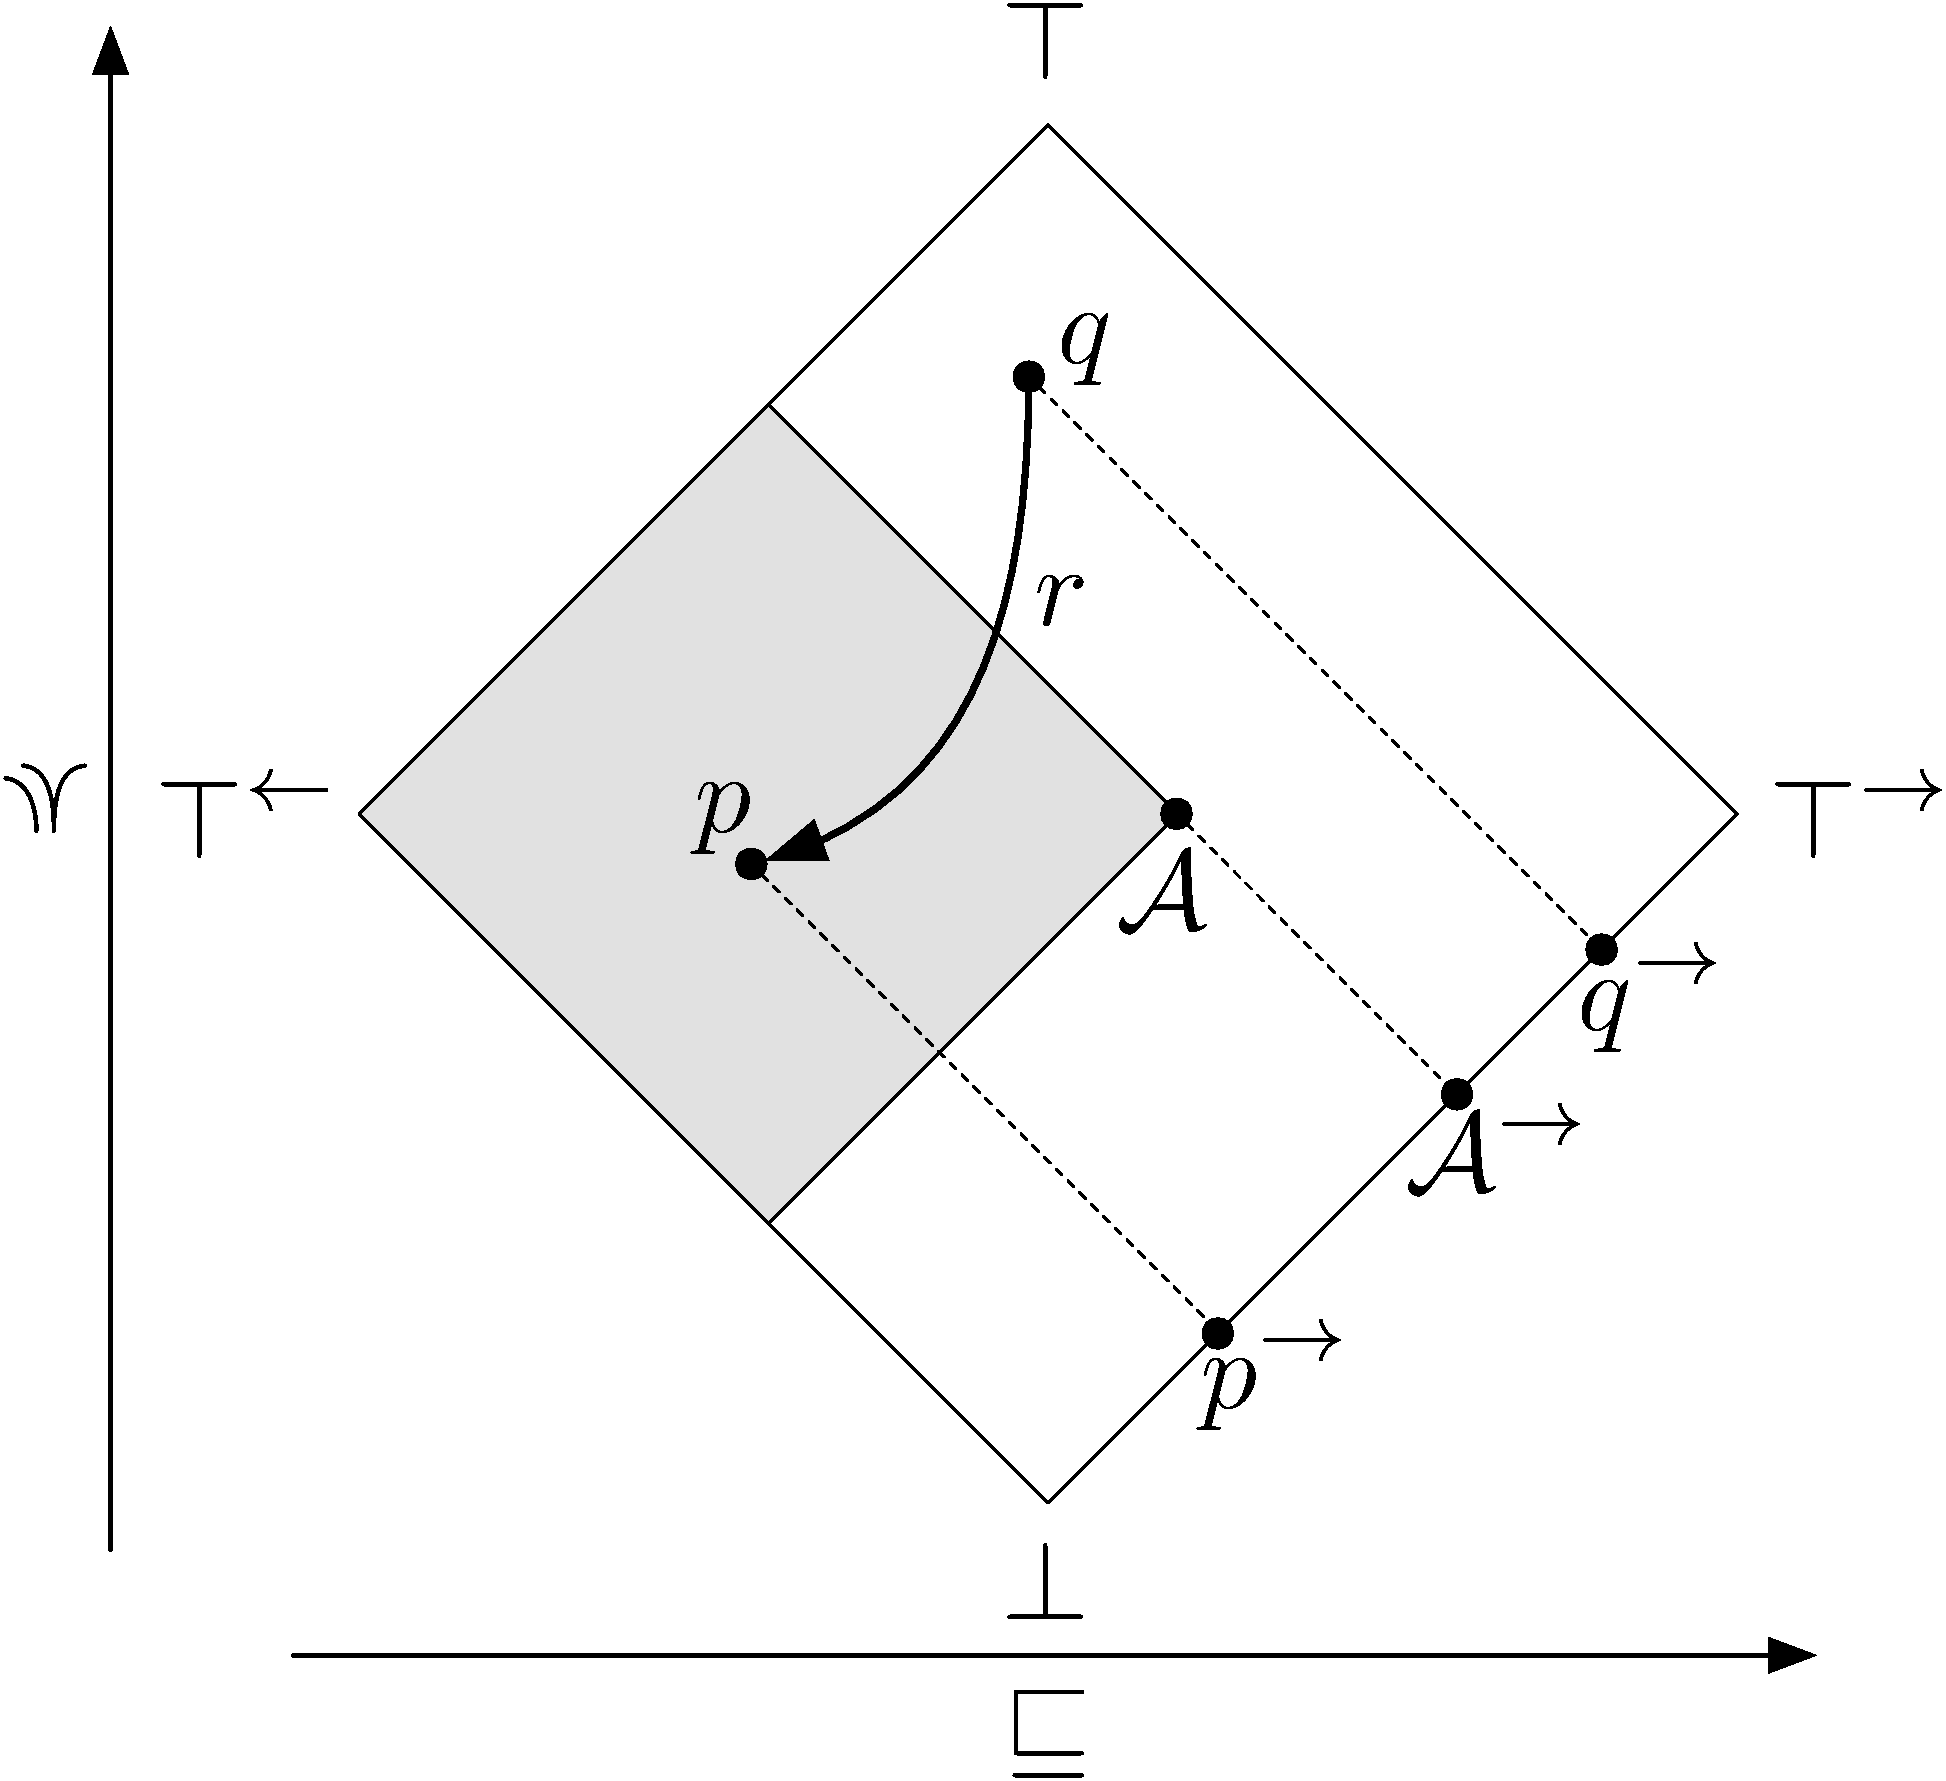
\includegraphics[scale=0.25]{Illustrations/bad-flow.pdf}
    \caption{Information labeled with principal $q$, which previously could not be relabeled as $\Attacker$, can now be relabeled as $p$. This information can, in turn, now be relabeled as $\Attacker$.}
    \label{fig:bad-release}
\end{figure}

\paragraph{Low-equivalence}
We define a low-equivalence relation that makes explicit which traces and memories an attacker can distinguish. As both traces and memories contain expressions, we start by defining a low-equivalence on expressions. Figure~\ref{fig:low-eq-expr} shows an excerpt of the low-equivalence relation on expressions. Rule \ruleref{Low-Eq-High} states that any two expressions are low-equivalent in an environment with a current label that does not flow to the attacker. This idea is similar to the term erasure technique used in \cite{SRMMlio} and subsequent presentations of the LIO attacker model \cite{Stefan:2012:ACT:2364527.2364557, 10.1007/978-3-642-40203-6_40, 10.1007/978-3-319-24858-5_13}.

For most cases this judgment recursively inspects the subexpressions of each expression (as can be seen in \ruleref{Low-Eq-Abs}), but differ in a few cases. In order to relate dynamically allocated addresses we follow \cite{Banerjee:2002:SIF:794201.795164} and use a partial bijection $\bijection: \Addr \partialto \Addr$ in \ruleref{Low-Eq-Addr}. The most important rules are \ruleref{Low-Eq-Labeled-1} that makes explicit the notion that an attacker cannot distinguish two terms labeled with a principal which does not flow to the attacker, and \ruleref{Low-Eq-Labeled-2} which states that an attacker can ``look inside'' terms labeled with principals that flow to the attacker. When $\bijection$ is not important we write $\loweq{C}{\Attacker}{\expr_1}{\expr_2}$ to mean $\loweq{C}{\Attacker}[\bijection]{\expr_1}{\expr_2}$ for some bijection $\bijection$.

\begin{figure}
    \centering
    \begin{mathpar}
    \inferrule[Low-Eq-High]{\nopostnotflowstoquery{n; \env^i}{\env^i_n.\lblkw}{\Attacker}\\\\ i = 1,2}{\loweq{C}{\Attacker}[\bijection]{\expr_1}{\expr_2}}
    \and
    \inferrule[Low-Eq-Low]{\nopostflowstoquery{n; \env^i}{\env^i_n.\lblkw}{\Attacker}\\\\ i = 1,2 \and \loweql{C}{\Attacker}[\bijection]{\expr_1}{\expr_2}}{\loweq{C}{\Attacker}{\expr_1}{\expr_2}}
    \and
    \inferrule[Low-Eq-Addr]{\bijection(\addr_1) = \addr_2}{\loweql{C}{\Attacker}[\bijection]{\addr_1}{\addr_2}}
    \and
    \inferrule[Low-Eq-Abs]{\loweql{C}{\Attacker}[\bijection]{\expr_1}{\expr_2}}{\loweql{C}{\Attacker}[\bijection]{\abs{m}{\type}{x}{\expr_1}}{\abs{m}{\type}{x}{\expr_2}}}
    \and
    \inferrule[Low-Eq-Labeled-1]{\nopostnotflowstoquery{n; \env^i}{p_i}{\Attacker}\quad i = 1,2}{\loweql{C}{\Attacker}[\bijection]{\lb{p_1}{\expr_1}}{\lb{p_2}{\expr_2}}}
    \and
    \inferrule[Low-Eq-Labeled-2]{\nopostflowstoquery{n; \env^i}{q}{\Attacker}\\\\\ i = 1,2 \and \loweql{C}{\Attacker}[\bijection]{\expr_1}{\expr_2}}{\loweql{C}{\Attacker}[\bijection]{\lb{q}{\expr_1}}{\lb{q}{\expr_2}}}
    \end{mathpar}
    \caption{Low-equivalence for terms and expressions. The meta-variable $C$ abbreviates $n; \env^1; \env^2$.}
    \label{fig:low-eq-expr}
\end{figure}

The low-equivalence relation on expressions induces a low-equivalence relation on events, and low-equivalence of traces are defined as pairwise low-equivalence of the elements of the trace. We write $t_1 \simeq_{\Attacker}^{\bijection} t_2$ for the low-equivalence relation on traces, and $t_1 \simeq_{\Attacker} t_2$ to mean $t_1 \simeq_{\Attacker}^{\bijection} t_2$ for some bijection $\bijection$.

Finally, Figure~\ref{fig:low-eq-memories} shows low-equivalence on memories. Rule \ruleref{Store-Eq-Empty} states that two empty stores are low-equivalent, and rule \ruleref{Store-Eq-Low} states that extending two stores with low-equivalent expressions preserves low-equivalence. Lastly, rules \ruleref{Store-Eq-High-1} and \ruleref{Store-Eq-High-2} states that both stores can be extended with terms labeled with a principal that does not flow to $\Attacker$ without the attacker being able to distinguish the memories. We extend the notion of low-equivalence on stores to $\Nameset$-indexed sets of stores and write $\loweq{C}{\Attacker}[\bijection]{\globalstore}{\altglobalstore}$ when $\forall n \in \Nameset~.~ \loweq{C}{\Attacker}[\bijection]{\globalstore(n)}{\altglobalstore(n)}$.

To simplify the statement of our end-to-end security guarantee note that, for any $n, m \in \Nameset$ we have $\loweq{n; \emptyenv; \emptyenv}{\Attacker}{\store}{\altstore}$ if and only if $\loweq{m; \emptyenv; \emptyenv}{\Attacker}{\store}{\altstore}$. Thus, we write $\store \simeq_{\Attacker} \altstore$ to mean $\loweq{n; \emptyenv; \emptyenv}{\Attacker}{\store}{\altstore}$ for some $n$.

\begin{figure}
    \centering
    \begin{mathpar}
    \inferrule[Store-Eq-Empty]{~}{\loweq{C}{\Attacker}[\bijection]{\varnothing}{\varnothing}}
    \and
    \inferrule[Store-Eq-Low]{\bijection(\addr_1) = \addr_2 \and \loweq{C}{\Attacker}[\bijection]{\expr_1}{\expr_2} \\\\ \nopostflowstoquery{n; \env^i}{q}{\Attacker}\quad i = 1,2 \\\\ \loweq{C}{\Attacker}[\bijection]{\store_1}{\store_2} \\\\ \store_i' = \extend{\store_i}{\addr_i}{(\lb{q}{\expr_i})}}{\loweq{C}{\Attacker}[\bijection]{\store_1'}{\store_2'}}
    \and
    \inferrule[Store-Eq-High-1]{\nopostnotflowstoquery{n; \env^1}{q}{\Attacker} \\\\ \loweq{C}{\Attacker}[\bijection]{\store_1}{\store_2}}{\loweq{C}{\Attacker}[\bijection]{\extend{\store_1}{\addr}{\lb{q}{\expr}}}{\store_2}}
    \and
    \inferrule[Store-Eq-High-2]{\nopostnotflowstoquery{n; \env^2}{q}{\Attacker} \\\\ \loweq{C}{\Attacker}[\bijection]{\store_1}{\store_2}}{\loweq{C}{\Attacker}[\bijection]{\store_1}{\extend{\store_2}{\addr}{\lb{q}{\expr}}}}
    \end{mathpar}
    \caption{Low-equivalence for memories. The meta-variable $C$ abbreviates $n; \env^1; \env^2$.}
    \label{fig:low-eq-memories}
\end{figure}

\paragraph{Attacker knowledge}
We present our noninterference result using the notion of attacker knowledge \cite{Askarov:2008:TNL:1462455.1462485, 4223226}. The attacker's knowledge is the set of initial memories that could lead to a given observable trace, and a larger knowledge correspond to more uncertainty about the initial memory. Formally, an attacker's knowledge given a trace $t$ produced by expression $\expr$ and the initial set of memories $\globalstore$ is the set
\begin{equation*}
k^n_{\Attacker}(\globalstore, \expr, t) = \left\{ \, \altglobalstore \, \middle\vert \, \globalstore \simeq_{\Attacker} \altglobalstore \wedge \, \gconfig{n}{\emptyenv}{S} \gstepstos[][\Attacker \filtertrace t'] \wedge \, t \simeq_{\Attacker} t' \, \right\}
\end{equation*}
where $S(m) = \config{\altglobalstore(n)}{\llbracket \expr \rrbracket_n(m)}$ and
\begin{equation*}
\llbracket \expr \rrbracket_n(m) =
\begin{cases}
\expr & \text{ if } n = m\\
\termsym & \text{ otherwise }
\end{cases}
\end{equation*}

and the policy \cite{6234468} is defined as all possible terminating memories
\begin{equation*}
k^n_{\Attacker}(\globalstore, \expr) = \left\{ \,\altglobalstore \, \middle\vert \, \globalstore \simeq_{\Attacker} \altglobalstore \wedge \, \gconfig{n}{\emptyenv}{S} \gstepstos \, \right\}
\end{equation*}
where $S(m) = \config{\altglobalstore(n)}{\llbracket \expr \rrbracket_n(m)}$. We can now state termination-insensitive noninterference for \lang{} as follows.

\begin{theorem}[Noninterference]\label{thm:ni}
Let $\expr$ satisfy $\hastype{n; \tenv}{\expr}{\type}$.
If $\gconfig{n}{\varnothing}{S} \gstepstos[][A \filtertrace t]$ for $S(m) = \config{\globalstore(m)}{\llbracket \expr \rrbracket_n(m)}$ such that $\good{A}{t}$ then $k^n_{\Attacker}(\globalstore, \expr, t) \supseteq k^n_{\Attacker}(\globalstore, \expr)$.
\end{theorem}

Theorem~\ref{thm:ni} is proved using a generalized version of the statement that quantifies over any two low-equivalent global configurations and proving that they emit low-equivalent observable traces. An important invariant obtained by quantifying only over good traces is that whenever $\actsforquery{n; \env_1}{p}{q}{\level}$ and $\nopostflowstoquery{n; \env_1}{\level}{\Attacker}$ it holds that $\actsforquery{n; \env_2}{p}{q}{\level}$ and $\nopostflowstoquery{n; \env_2}{\level}{\Attacker}$. The technical report \cite{techreport} contains a complete proof of Theorem~\ref{thm:ni}.

\TODO{Also talk about how raising the current label is a side-channel that we close in our system.}